\hypertarget{seguranuxe7a-em-sistemas-scada}{%
\chapter{Segurança em Sistemas SCADA}\label{seguranuxe7a-em-sistemas-scada}}

\section*{Objetivos de Aprendizagem}

Ao final deste capítulo, o leitor será capaz de:

\begin{itemize}
\tightlist
\item
  Compreender por que a cibersegurança em OT é diferente da segurança em TI.
\item
  Identificar as principais ameaças e vetores de ataque a sistemas SCADA.
\item
  Aplicar os conceitos da norma IEC 62443 para proteção de ambientes industriais.
\item
  Descrever as melhores práticas de segmentação de redes TI/OT.
\end{itemize}

\begin{center}\rule{0.5\linewidth}{0.5pt}\end{center}

\hypertarget{ot-security-por-que-uxe9-diferente}{%
\section{OT Security: Por que é Diferente?}\label{ot-security-por-que-uxe9-diferente}}

A cibersegurança em \textbf{OT} (\emph{Operational Technology}) segue princípios distintos da segurança em \textbf{TI} (\emph{Information Technology}). A tríade clássica de segurança \textbf{CIA} (Confidencialidade, Integridade, Disponibilidade) tem pesos diferentes:

\textbf{Tabela 8.1 -- Prioridades CIA: TI \ensuremath{\times} OT}

\begin{longtable}[]{@{}lll@{}}
\toprule\noalign{}
Prioridade & TI (Corporativa) & OT (Industrial) \\
\midrule\noalign{}
\endhead
\bottomrule\noalign{}
\endlastfoot
\textbf{1ª} & Confidencialidade & \textbf{Disponibilidade} \\
\textbf{2ª} & Integridade & \textbf{Integridade} \\
\textbf{3ª} & Disponibilidade & Confidencialidade \\
\end{longtable}

Na OT, \textbf{parar um sistema pode significar:} explosão em uma refinaria, blackout em uma cidade, contaminação de abastecimento de água, acidentes com operadores. A segurança das \textbf{pessoas} e do \textbf{processo} está acima da confidencialidade dos dados.

\textbf{Outras diferenças críticas:}

\begin{itemize}
\tightlist
\item
  \textbf{Ciclo de vida:} sistemas OT operam por décadas; patches e atualizações são raros ou impossíveis sem parada programada.
\item
  \textbf{Tempo real:} latências introduzidas por firewalls e antivírus podem afetar o controle.
\item
  \textbf{Protocolos legados:} Modbus, DNP3 e outros foram projetados sem autenticação ou criptografia.
\item
  \textbf{Air gap histórico:} sistemas OT eram fisicamente isolados; a convergência TI/OT eliminou essa barreira.
\end{itemize}

\begin{caixaatencao}

\textbf{Atenção:} Um antivírus mal configurado em um servidor SCADA pode consumir CPU durante um scan e causar timeouts de comunicação --- resultando em falsos alarmes ou perda de controle do processo. Soluções de segurança para OT devem ser \textbf{específicas para o ambiente industrial}.

\end{caixaatencao}

\begin{center}\rule{0.5\linewidth}{0.5pt}\end{center}

\hypertarget{linha-do-tempo-de-ataques-a-infraestruturas-cruxedticas}{%
\section{Linha do Tempo de Ataques a Infraestruturas Críticas}\label{linha-do-tempo-de-ataques-a-infraestruturas-cruxedticas}}

\begin{caixafigura}

\textbf{{[}Figura 8.1 -- Linha do tempo de ataques a sistemas SCADA e infraestruturas críticas{]}}
\emph{Infográfico com os principais incidentes de segurança em OT: Stuxnet (2010), Ukraine Power Grid (2015, 2016), Triton/Trisis (2017), Colonial Pipeline (2021), Oldsmar Water Treatment (2021). Para cada evento: ano, país, setor afetado, impacto e vetor de ataque.}

\end{caixafigura}

\textbf{Stuxnet (2010):} malware sofisticado criado para sabotar centrífugas de enriquecimento de urânio no Irã, manipulando CLPs Siemens S7-315/417. Primeiro ataque cibernético documentado a causar dano físico real.

\textbf{Ukraine Power Grid (2015):} ataque via phishing comprometeu estações SCADA de distribuidoras de energia, resultando em blackout para 230.000 pessoas.

\textbf{Triton/Trisis (2017):} ataque direcionado a sistemas de segurança funcional (SIS --- Safety Instrumented System) em uma refinaria petroquímica no Oriente Médio. O objetivo era desabilitar a proteção que impede explosões.

\textbf{Colonial Pipeline (2021):} ransomware no sistema de TI da maior operadora de oleodutos dos EUA. A empresa desligou preventivamente o SCADA --- causando escassez de combustível na Costa Leste americana.

\begin{center}\rule{0.5\linewidth}{0.5pt}\end{center}

\hypertarget{principais-vetores-de-ataque}{%
\section{Principais Vetores de Ataque}\label{principais-vetores-de-ataque}}

\begin{longtable}[]{@{}
  >{\raggedright\arraybackslash}p{(\columnwidth - 4\tabcolsep) * \real{0.3333}}
  >{\raggedright\arraybackslash}p{(\columnwidth - 4\tabcolsep) * \real{0.3333}}
  >{\raggedright\arraybackslash}p{(\columnwidth - 4\tabcolsep) * \real{0.3333}}@{}}
\toprule\noalign{}
\begin{minipage}[b]{\linewidth}\raggedright
Vetor
\end{minipage} & \begin{minipage}[b]{\linewidth}\raggedright
Descrição
\end{minipage} & \begin{minipage}[b]{\linewidth}\raggedright
Mitigação
\end{minipage} \\
\midrule\noalign{}
\endhead
\bottomrule\noalign{}
\endlastfoot
Phishing & Email falso induz operador a instalar malware & Treinamento, MFA, filtro de email \\
USB / mídia removível & Malware em pen drives usados na rede OT & Política zero USB, portas bloqueadas \\
Acesso remoto inseguro & VPN sem MFA, RDP exposto & MFA obrigatório, jump server, PAM \\
Vulnerabilidades em sistemas legados & CLPs/HMIs sem patch por anos & Segmentação, monitoramento passivo \\
Supply chain & Firmware malicioso em hardware comprado & Verificação de integridade, fornecedores certificados \\
Movimento lateral TI\ensuremath{\rightarrow}OT & Atacante compromete TI e se move para OT & Segmentação, DMZ industrial \\
\end{longtable}

\begin{center}\rule{0.5\linewidth}{0.5pt}\end{center}

\hypertarget{norma-iec-62443}{%
\section{Norma IEC 62443}\label{norma-iec-62443}}

A \textbf{IEC 62443} (\emph{Security for Industrial Automation and Control Systems}) é a família de normas internacional para cibersegurança em sistemas de automação e controle industrial. É estruturada em quatro séries:

\begin{longtable}[]{@{}
  >{\raggedright\arraybackslash}p{(\columnwidth - 4\tabcolsep) * \real{0.3333}}
  >{\raggedright\arraybackslash}p{(\columnwidth - 4\tabcolsep) * \real{0.3333}}
  >{\raggedright\arraybackslash}p{(\columnwidth - 4\tabcolsep) * \real{0.3333}}@{}}
\toprule\noalign{}
\begin{minipage}[b]{\linewidth}\raggedright
Série
\end{minipage} & \begin{minipage}[b]{\linewidth}\raggedright
Título
\end{minipage} & \begin{minipage}[b]{\linewidth}\raggedright
Conteúdo
\end{minipage} \\
\midrule\noalign{}
\endhead
\bottomrule\noalign{}
\endlastfoot
\textbf{IEC 62443-1} & Geral & Terminologia, conceitos, modelos \\
\textbf{IEC 62443-2} & Políticas e Procedimentos & Requisitos para operadores e integradores \\
\textbf{IEC 62443-3} & Sistema & Avaliação de risco, zonas e condutos \\
\textbf{IEC 62443-4} & Componentes & Requisitos para produtos (CLPs, SCADA) \\
\end{longtable}

\hypertarget{zonas-de-seguranuxe7a-e-condutos}{%
\subsection{Zonas de Segurança e Condutos}\label{zonas-de-seguranuxe7a-e-condutos}}

O conceito central da IEC 62443-3-2 é dividir o sistema em \textbf{zonas} (\emph{Security Zones}) e \textbf{condutos} (\emph{Conduits}):

\begin{itemize}
\tightlist
\item
  \textbf{Zona de Segurança:} agrupamento de ativos com requisitos de segurança semelhantes e nível de confiança equivalente.
\item
  \textbf{Conduto:} canal de comunicação que conecta duas zonas, com controles de segurança aplicados ao tráfego.
\end{itemize}

\begin{center}
\IfFileExists{../figuras/capitulo-08-m1.pdf}{%
  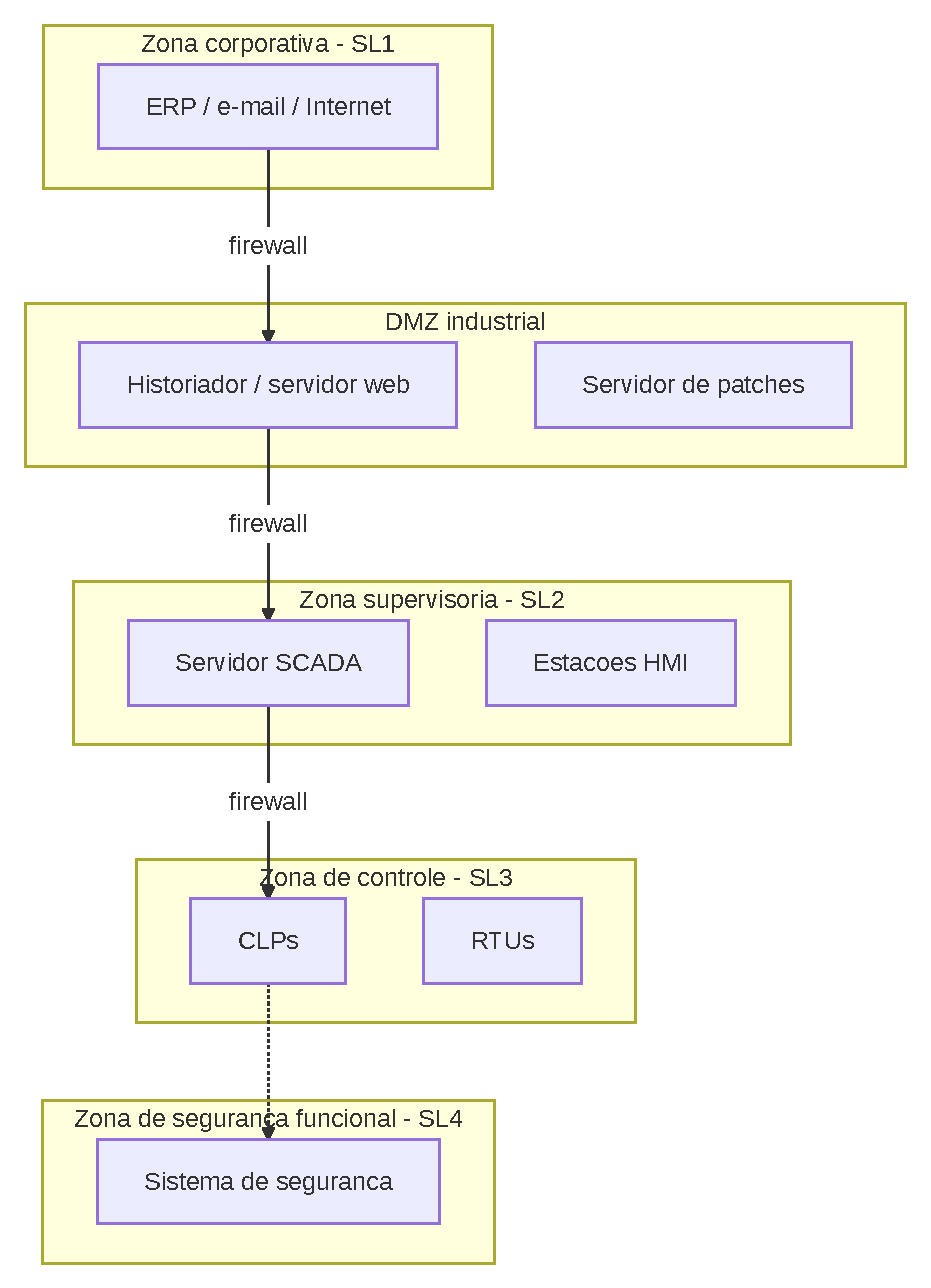
\includegraphics[width=\linewidth,height=0.8\textheight,keepaspectratio]{../figuras/capitulo-08-m1.pdf}%
}{\fbox{\parbox{0.9\linewidth}{\small Diagrama Mermaid ainda não renderizado: capitulo-08-m1. Rode scripts/render-mermaid.sh.}}}
\end{center}

\begin{caixafigura}

\textbf{{[}Figura 8.2 -- Modelo de zonas e condutos IEC 62443{]}}
\emph{Diagrama de zonas concêntricas ou em camadas: Zona Corporativa (exterior) \ensuremath{\rightarrow} DMZ Industrial \ensuremath{\rightarrow} Zona Supervisória \ensuremath{\rightarrow} Zona de Controle \ensuremath{\rightarrow} Zona de Segurança (centro, mais protegida). Firewalls e diodos de dados entre cada zona. Cores indicando nível de segurança crescente.}

\end{caixafigura}

\hypertarget{security-levels-sl}{%
\subsection{Security Levels (SL)}\label{security-levels-sl}}

A norma define quatro \textbf{Níveis de Segurança} (\emph{Security Level}):

\begin{longtable}[]{@{}
  >{\raggedright\arraybackslash}p{(\columnwidth - 4\tabcolsep) * \real{0.3333}}
  >{\raggedright\arraybackslash}p{(\columnwidth - 4\tabcolsep) * \real{0.3333}}
  >{\raggedright\arraybackslash}p{(\columnwidth - 4\tabcolsep) * \real{0.3333}}@{}}
\toprule\noalign{}
\begin{minipage}[b]{\linewidth}\raggedright
SL
\end{minipage} & \begin{minipage}[b]{\linewidth}\raggedright
Proteção contra
\end{minipage} & \begin{minipage}[b]{\linewidth}\raggedright
Descrição
\end{minipage} \\
\midrule\noalign{}
\endhead
\bottomrule\noalign{}
\endlastfoot
\textbf{SL 1} & Causas não intencionais & Erros humanos, falhas acidentais \\
\textbf{SL 2} & Atacantes com baixa habilidade e motivação & Script kiddies, ataques oportunistas \\
\textbf{SL 3} & Atacantes sofisticados, motivados & Hackers patrocinados por concorrentes \\
\textbf{SL 4} & Atores estatais, recursos ilimitados & Ataques como Stuxnet \\
\end{longtable}

\begin{center}\rule{0.5\linewidth}{0.5pt}\end{center}

\hypertarget{boas-pruxe1ticas-de-seguranuxe7a-em-scada}{%
\section{Boas Práticas de Segurança em SCADA}\label{boas-pruxe1ticas-de-seguranuxe7a-em-scada}}

\hypertarget{segmentauxe7uxe3o-de-redes}{%
\subsection{Segmentação de Redes}\label{segmentauxe7uxe3o-de-redes}}

\begin{caixafigura}

\textbf{{[}Figura 8.3 -- Segmentação em zonas, com o tráfego permitido e o bloqueado{]}}
\emph{Diagrama de blocos com quatro zonas empilhadas (corporativa, DMZ industrial, supervisória e de controle), mostrando as setas de tráfego permitido e as bloqueadas. Anotar junto a cada seta o protocolo e a porta, e destacar os pontos de inspeção: firewall industrial e proxy reverso. Incluir legenda com o nível de segurança (SL) de cada zona.}

\end{caixafigura}

\begin{itemize}
\tightlist
\item
  Isolar completamente a rede OT da rede corporativa com \textbf{firewall industrial} (ex.: Fortinet FortiGate, Cisco ASA, Schneider Electric ConneXium).
\item
  Criar \textbf{DMZ Industrial} para sistemas que precisam compartilhar dados com TI (historiador, servidor web de relatórios).
\item
  Usar \textbf{diodos de dados} (\emph{data diodes}) em pontos onde apenas fluxo unidirecional é necessário --- fisicamente impossível de hackear de volta.
\end{itemize}

\hypertarget{controle-de-acesso-remoto}{%
\subsection{Controle de Acesso Remoto}\label{controle-de-acesso-remoto}}

\begin{itemize}
\tightlist
\item
  \textbf{VPN com MFA} (\emph{Multi-Factor Authentication}) para todos os acessos remotos.
\item
  \textbf{Jump Server / Bastion Host:} toda conexão remota passa por um servidor intermediário --- nunca acesso direto a CLPs.
\item
  \textbf{PAM} (\emph{Privileged Access Management}): registro e gravação de todas as sessões de manutenção remota.
\item
  \textbf{Tempo limitado:} acessos remotos habilitados apenas durante janelas de manutenção, com aprovação.
\end{itemize}

\begin{caixadica}

\textbf{Dica:} Nunca exponha a porta RDP (3389) ou SSH (22) de servidores SCADA diretamente para a internet. Uma busca no Shodan.io revela milhares de sistemas SCADA acessíveis publicamente --- a maioria sem autenticação adequada.

\end{caixadica}

\hypertarget{gestuxe3o-de-vulnerabilidades-e-patches}{%
\subsection{Gestão de Vulnerabilidades e Patches}\label{gestuxe3o-de-vulnerabilidades-e-patches}}

\begin{itemize}
\tightlist
\item
  \textbf{Inventário de ativos:} manter catálogo atualizado de todos os equipamentos OT (fabricante, modelo, firmware, protocolos).
\item
  \textbf{Avaliação de vulnerabilidades passiva:} ferramentas como \textbf{Claroty}, \textbf{Dragos} ou \textbf{Tenable OT} identificam vulnerabilidades sem enviar pacotes ativos (que poderiam impactar o processo).
\item
  \textbf{Patch em janelas de manutenção:} atualizações testadas em ambiente de homologação antes da produção.
\item
  \textbf{EOL Management:} equipamentos sem suporte (End-of-Life) devem ser isolados e substituídos no prazo.
\end{itemize}

\hypertarget{backup-e-recuperauxe7uxe3o}{%
\subsection{Backup e Recuperação}\label{backup-e-recuperauxe7uxe3o}}

\begin{itemize}
\tightlist
\item
  Backup regular de: configurações de CLPs, configurações do SCADA (tags, telas, scripts), banco de dados histórico.
\item
  Teste periódico de restauração.
\item
  Plano de \textbf{DRP} (\emph{Disaster Recovery Plan}) específico para o ambiente OT.
\end{itemize}

\hypertarget{treinamento-e-cultura-de-seguranuxe7a}{%
\subsection{Treinamento e Cultura de Segurança}\label{treinamento-e-cultura-de-seguranuxe7a}}

\begin{itemize}
\tightlist
\item
  Operadores e técnicos de manutenção são o principal vetor de ataque (phishing, USB).
\item
  Treinamentos regulares de \textbf{segurança cibernética industrial} para toda a equipe OT.
\item
  Política clara sobre uso de dispositivos pessoais e mídias removíveis na planta.
\end{itemize}

\begin{caixanota}

\textbf{Nota:} No Brasil, o setor de energia elétrica é regulado pela \textbf{Resolução Normativa ANEEL nº 964/2021}, que estabelece requisitos mínimos de segurança cibernética para o Ambiente de TI e OT de agentes do setor elétrico, baseados na IEC 62443 e no NIST Cybersecurity Framework.

\end{caixanota}

\begin{center}\rule{0.5\linewidth}{0.5pt}\end{center}

\hypertarget{monitoramento-e-resposta-a-incidentes-soc-ot}{%
\section{Monitoramento e Resposta a Incidentes (SOC OT)}\label{monitoramento-e-resposta-a-incidentes-soc-ot}}

Responder a um incidente em rede industrial é diferente de responder em rede corporativa: não se
pode simplesmente desligar o equipamento suspeito se ele estiver operando o processo.

\begin{center}
\IfFileExists{../figuras/capitulo-08-m2.pdf}{%
  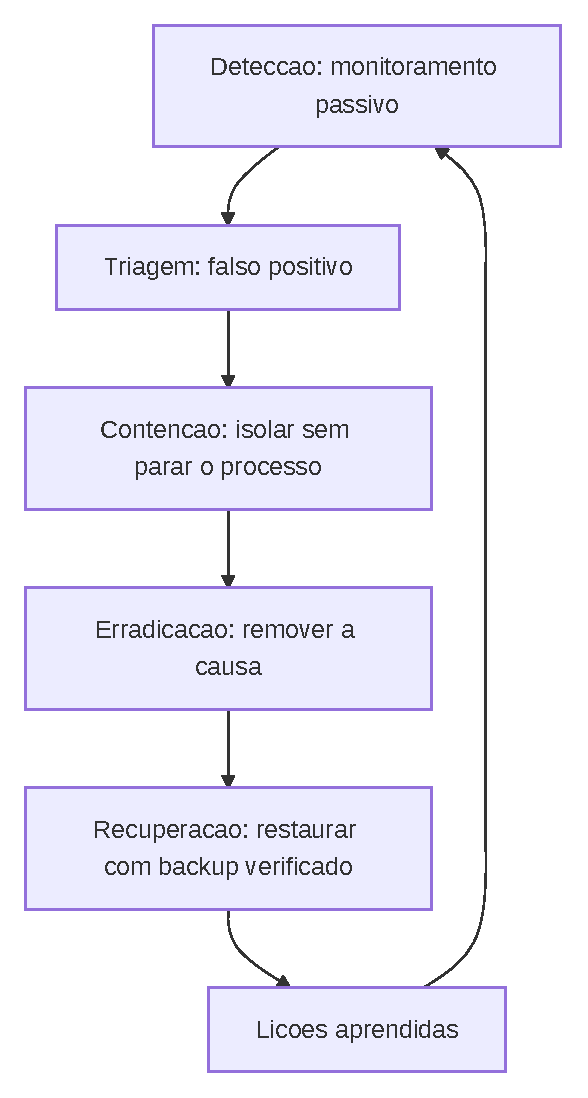
\includegraphics[width=\linewidth,height=0.8\textheight,keepaspectratio]{../figuras/capitulo-08-m2.pdf}%
}{\fbox{\parbox{0.9\linewidth}{\small Diagrama Mermaid ainda não renderizado: capitulo-08-m2. Rode scripts/render-mermaid.sh.}}}
\end{center}

\hypertarget{monitoramento-passivo-da-rede-ot}{%
\subsection{Monitoramento Passivo da Rede OT}\label{monitoramento-passivo-da-rede-ot}}

Ferramentas de monitoramento OT analisam o tráfego de rede de forma \textbf{passiva} --- sem injetar pacotes --- para:

\begin{itemize}
\tightlist
\item
  Criar inventário automático de ativos (dispositivo, firmware, protocolo).
\item
  Detectar comunicações anômalas (CLP falando com IP desconhecido, volume atípico de dados).
\item
  Alertar sobre tentativas de varredura de rede.
\end{itemize}

\textbf{Soluções especializadas em OT:}

\begin{longtable}[]{@{}
  >{\raggedright\arraybackslash}p{(\columnwidth - 4\tabcolsep) * \real{0.3333}}
  >{\raggedright\arraybackslash}p{(\columnwidth - 4\tabcolsep) * \real{0.3333}}
  >{\raggedright\arraybackslash}p{(\columnwidth - 4\tabcolsep) * \real{0.3333}}@{}}
\toprule\noalign{}
\begin{minipage}[b]{\linewidth}\raggedright
Ferramenta
\end{minipage} & \begin{minipage}[b]{\linewidth}\raggedright
Empresa
\end{minipage} & \begin{minipage}[b]{\linewidth}\raggedright
Diferencial
\end{minipage} \\
\midrule\noalign{}
\endhead
\bottomrule\noalign{}
\endlastfoot
Claroty & Claroty & Amplo suporte a protocolos OT; integração com SIEM \\
Dragos & Dragos & Threat intelligence focado em OT (grupos de ameaça) \\
Tenable OT & Tenable & Integração com gestão de vulnerabilidades TI \\
Microsoft Defender for IoT & Microsoft & Integrado ao Azure Sentinel \\
Nozomi Networks & Nozomi & IA para detecção de anomalias OT \\
\end{longtable}

\hypertarget{plano-de-resposta-a-incidentes-ot}{%
\subsection{Plano de Resposta a Incidentes OT}\label{plano-de-resposta-a-incidentes-ot}}

Em caso de incidente cibernético em ambiente OT:

\begin{enumerate}
\def\labelenumi{\arabic{enumi}.}
\tightlist
\item
  \textbf{Detecção:} sistema de monitoramento alerta sobre atividade suspeita.
\item
  \textbf{Avaliação:} equipe de segurança avalia se é falso positivo ou ameaça real.
\item
  \textbf{Contenção:} isolar segmento afetado sem parar o processo (se possível).
\item
  \textbf{Erradicação:} remover o malware ou fechar o vetor de ataque.
\item
  \textbf{Recuperação:} restaurar sistemas a partir de backup limpo; testar antes de retornar à produção.
\item
  \textbf{Lições aprendidas:} documentar o incidente; atualizar procedimentos.
\end{enumerate}

\begin{center}\rule{0.5\linewidth}{0.5pt}\end{center}

\hypertarget{estudo-de-caso-segmentauxe7uxe3o-por-zonas-e-condutos-em-uma-planta-de-muxe9dio-porte}{%
\section{\texorpdfstring{Estudo de Caso --- Segmentação por zonas e condutos em uma planta de médio porte}{Estudo de Caso  Segmentação por zonas e condutos em uma planta de médio porte}}\label{estudo-de-caso-segmentauxe7uxe3o-por-zonas-e-condutos-em-uma-planta-de-muxe9dio-porte}}

\textbf{Cenário.} Planta de processamento contínuo com 340 funcionários. A rede de automação cresceu
por acumulação ao longo de 15 anos: CLPs, IHM, supervisório, servidor de histórico, estações de
engenharia e o Wi-Fi da manutenção dividem hoje o mesmo conjunto de \emph{switches}, com o roteador
corporativo ligado a um deles. Não há documentação de endereçamento.

\textbf{Diagnóstico pelo modelo de zonas e condutos (IEC 62443).} O primeiro produto do trabalho não é
um firewall: é o \textbf{inventário de ativos com função e criticidade}. Só depois as zonas aparecem.

\begin{longtable}[]{@{}
  >{\raggedright\arraybackslash}p{(\columnwidth - 4\tabcolsep) * \real{0.3333}}
  >{\raggedright\arraybackslash}p{(\columnwidth - 4\tabcolsep) * \real{0.3333}}
  >{\raggedright\arraybackslash}p{(\columnwidth - 4\tabcolsep) * \real{0.3333}}@{}}
\toprule\noalign{}
\begin{minipage}[b]{\linewidth}\raggedright
Zona proposta
\end{minipage} & \begin{minipage}[b]{\linewidth}\raggedright
Ativos
\end{minipage} & \begin{minipage}[b]{\linewidth}\raggedright
Nível de criticidade
\end{minipage} \\
\midrule\noalign{}
\endhead
\bottomrule\noalign{}
\endlastfoot
Zona de controle & CLPs, IHM locais, \emph{drives} & Crítica --- para a produção se parar \\
Zona de supervisão & Servidores SCADA e historiador, estações de operação & Crítica \\
Zona de engenharia & Estações de programação, \emph{notebooks} de fornecedor & Alta \\
Zona corporativa & ERP, e-mail, estações administrativas & Média \\
Zona de acesso remoto & VPN de fornecedores e acesso de manutenção & Alta, com sessão auditada \\
\end{longtable}

\textbf{Regras de conduto que fizeram a diferença.} A segmentação só reduz risco quando o tráfego entre
zonas é \textbf{explícito}:

\begin{itemize}
\tightlist
\item
  Supervisão \textbf{lê} do controle; o controle \textbf{não inicia} conexão para a supervisão.
\item
  Engenharia acessa o controle apenas em janela agendada, com sessão gravada.
\item
  Corporativo \textbf{nunca} alcança o controle diretamente --- inclusive o tráfego de atualização de
  \emph{antivírus}, que costuma ser o furo silencioso das segmentações.
\item
  Nenhum acesso remoto entra sem duplo fator e sem registro de sessão.
\end{itemize}

\textbf{O que observar no resultado.} A segmentação \textbf{não} exige trocar CLP nem parar a produção: as
zonas são implementadas em VLANs e regras de firewall, com janelas de manutenção para repassar a
rede. O ganho maior, porém, costuma ser indireto: o inventário de ativos gerado na etapa 1 é o que
permite, depois, aplicar correções e detectar anomalias de tráfego.

\textbf{Limitações do arranjo.} Segmentar sem monitorar deixa o sistema mais difícil de operar e não
mais seguro --- a rede fica opaca, e cada diagnóstico passa a depender de alguém com acesso ao
firewall. A segmentação precisa vir acompanhada de registro de tráfego nas fronteiras de zona
(Seção 8.6).

\begin{center}\rule{0.5\linewidth}{0.5pt}\end{center}

\hypertarget{resumo}{%
\section{Resumo}\label{resumo}}

\begin{itemize}
\tightlist
\item
  Segurança OT prioriza \textbf{disponibilidade} acima de confidencialidade --- ao contrário da TI.
\item
  Sistemas SCADA foram projetados para disponibilidade, não para segurança; a convergência TI/OT os expôs a ameaças digitais.
\item
  A \textbf{IEC 62443} estrutura a segurança industrial em zonas, condutos e níveis de segurança (SL1--SL4).
\item
  Boas práticas essenciais: segmentação de rede, DMZ industrial, VPN com MFA, monitoramento passivo e treinamento de operadores.
\item
  Ferramentas especializadas como Claroty e Dragos permitem monitoramento OT sem impactar o processo.
\end{itemize}

\begin{center}\rule{0.5\linewidth}{0.5pt}\end{center}

\hypertarget{questuxf5es-de-revisuxe3o}{%
\section{Questões de Revisão}\label{questuxf5es-de-revisuxe3o}}

\textbf{Conceituais:}

\begin{enumerate}
\def\labelenumi{\arabic{enumi}.}
\tightlist
\item
  Por que a prioridade de segurança em OT (Disponibilidade \textgreater{} Integridade \textgreater{} Confidencialidade) é inversa à de TI?
\item
  O que são ``zonas de segurança'' e ``condutos'' na IEC 62443? Cite dois exemplos de cada um.
\item
  Por que o antivírus convencional de TI pode ser inadequado para servidores SCADA?
\end{enumerate}

\textbf{Práticas:}

\begin{enumerate}
\def\labelenumi{\arabic{enumi}.}
\setcounter{enumi}{3}
\tightlist
\item
  Uma empresa petroquímica conectou sua rede OT diretamente à rede corporativa para facilitar o acesso ao historiador a partir do ERP. Identifique os riscos dessa arquitetura e proponha uma solução com DMZ industrial.
\item
  Um técnico de manutenção precisa acessar remotamente um CLP para realizar ajuste de parâmetros fora do horário comercial. Descreva o procedimento seguro de acesso remoto, incluindo autenticação, registro e controle de sessão.
\end{enumerate}

\textbf{Desafio:}

\begin{enumerate}
\def\labelenumi{\arabic{enumi}.}
\setcounter{enumi}{5}
\tightlist
\item
  Com base no incidente do Stuxnet (2010), analise: (a) Qual era o objetivo do ataque? (b) Qual vetor de infecção foi usado? (c) Como ele manipulou os CLPs Siemens? (d) Quais medidas de segurança da IEC 62443 poderiam ter dificultado ou impedido o ataque?
\end{enumerate}

\begin{center}\rule{0.5\linewidth}{0.5pt}\end{center}

\hypertarget{referuxeancias}{%
\section{Referências}\label{referuxeancias}}

\begin{itemize}
\tightlist
\item
  IEC 62443: \emph{Security for Industrial Automation and Control Systems} (séries 1 a 4). IEC, 2018--2023.
\item
  NIST SP 800-82 Rev.~3: \emph{Guide to OT Security}. NIST, 2023.
\item
  ANEEL Resolução Normativa nº 964/2021. Disponível em: aneel.gov.br.
\item
  LANGNER, R. \emph{Stuxnet: Dissecting a Cyberwarfare Weapon}. IEEE Security \& Privacy, 2011.
\item
  CLAROTY. \emph{State of XIoT Security Report}. Disponível em: \url{claroty.com/research}.
\end{itemize}
